\makeheading{Lecture 7 | 2020-09-27}
\section{Independence}
\begin{Definition}{Independent}{}
    For any two random variables, we say $ X $ and $ Y $
    are \textbf{independent} if and only if
    \[ \Prob{X\in A,Y\in B}=\Prob{X\in A} \Prob{Y\in B} \]
    for any two sets $ A $ and $ B $ of real numbers.
\end{Definition}

\begin{Theorem}{Independent Random Variables}{}
    Suppose $ X $ and $ Y $ are random variables. $ X $
    and $ Y $ are independent if and only if
    \begin{enumerate}[label=(\arabic*)]
        \item $ F(x,y)=F_1(x)F_2(y) $, or
        \item $ f(x,y)=f_1(x)f_2(y) $.
    \end{enumerate}
\end{Theorem}

\begin{Theorem}{}{}
    Let $ g $ and $ h $ be real-valued functions.
    If $ X $ and $ Y $ are independent,
    then $ g(X) $ and $ h(Y) $ are independent.
\end{Theorem}

\begin{Example}{}{}
    If $ X $ and $ Y $ are independent,
    then $ X^2 $ and $ Y^2 $ are independent. However,
    if $ X^2 $ and $ Y^2 $ are independent, then $ X $
    and $ Y $ may not be independent. Can you find an example here?
    Choose $ X $ where
    \[ \Prob{X=1}
        =\Prob{X=-1}=\frac{1}{2} \]
\end{Example}

\begin{Example}{}{}
    Consider the joint discrete random variable
    $ f(x,y)=q^2 p^{x+y} $, where $ x=0,1,\ldots $
    and $ y=0,1,2,\ldots $. Then $ f_1(x)=qp^x $
    and $ f_2(y)=qp^y $. Therefore,
    $ f(x,y)=f_1(x)f_2(y) $
    shows that $ X $ and $ Y $ are independent.

    Consider $ \displaystyle
        f(x,y)=\begin{cases}
            x+y & 0\le x\le 1,\quad 0\le y\le 1 \\
            0   & \text{otherwise}
        \end{cases} $
    We've shown that
    \[ f_1(x)=\begin{dcases}
            x+\frac{1}{2} & 0\le x\le 1      \\
            0             & \text{otherwise}
        \end{dcases} \]
    \[ f_2(y)=\begin{dcases}
            y+\frac{1}{2} & 0\le y\le 1      \\
            0             & \text{otherwise}
        \end{dcases} \]
    We see that $ f(x,y)\neq f_1(x)f_2(y) $
    therefore, $ X $ and $ Y $ are not independent.
\end{Example}

\begin{Theorem}{Factorization Theorem for Independence}{}
    Suppose $ X $ and $ Y $ are random variables
    with joint probability (density) function $ f(x,y) $. Suppose
    also that $ A $ is the support set of $ (X,Y) $,
    $ A_1 $ is the support set of $ X $,
    and $ A_2 $ is the support set of $ Y $. Then
    $ X $ and $ Y $ are independent random variables
    if and only if there exist non-negative functions
    $ g(x) $ and $ h(y) $ such that
    \[ f(x,y)=g(x)h(y)\quad\forall(x,y)\in A_1\times A_2 \]
    where $ A_1\times A_2=\set{(x,y):x\in A_1,y\in A_2} $.
\end{Theorem}
\begin{Remark}{}{}
    Equivalently, we can check that both conditions are met:
    \begin{itemize}
        \item The support of $ A $ is a square or rectangle.
        \item The range of $ X $ does not depend on the values
              of $ y $ and the range of $ Y $ does not depend on the values of $ x $.
    \end{itemize}
\end{Remark}

\begin{Example}{}{}
    $ \displaystyle f(x,y)=\frac{\theta^{x+y}e^{-2\theta}}{x!y!} $
    where $ x,y\in\mathbb{Z}_{\ge 0} $. Are $ X $ and $ Y $
    independent or not? Find the marginal p.f.\ of $ X $ and $ Y $.

    \textbf{Solution.}
    \[ f(x,y)=\Uunderbracket{\frac{\theta^x}{x!} e^{-\theta}}_{g(x)}
        \Uunderbracket{\frac{\theta^y}{y!}e^{-\theta} }_{h(y)} \]
    The range of $ X $ does not depend on the value of $ y $. Therefore,
    $ X $ and $ Y $ are independent.
    \[ f_1(x)=\sum\limits_{y=0}^{\infty} f(x,y)=\frac{\theta^x e^{-\theta}}{x!}\quad x\in
        \mathbb{Z}_{\ge 0} \]
    \[ f_2(y)=\sum\limits_{x=0}^{\infty} f(x,y)=\frac{\theta^y e^{-\theta}}{y!}\quad y\in
        \mathbb{Z}_{\ge 0} \]
    If we've shown that $ X $ and $ Y $ are independent, then we can verify
    \[ f(x,y)=g(x)h(y) \]
    With $ f_1(x)=C_1 g(x) $ and $ f_2(y)=C_2 h(y) $
    where $ C_1,C_2\in\mathbb{R} $ is a constant. We know that $ C_1C_2=1 $.
\end{Example}

\begin{Example}{}{}
    If $ X $ and $ Y $ have joint p.d.f.\
    $ \displaystyle  f(x,y)=\frac{3}{2} y(1-x^2) $
    where $ -1\le x\le 1 $ and $ 0\le y\le 1 $.
    Are $ X $ and $ Y $ independent? Find $ f_1(x) $ and $ f_2(y) $.

    \textbf{Solution.}
    $ f(x,y)=\Uunderbracket{(1-x^2)}_{h(x)} \Uunderbracket{\frac{3}{2} y}_{g(y)} $
    and $ A =\set{(x,y):-1\le x\le 1,0\le y\le 1} $
    is a rectangle. Therefore $ X $ and $ Y $ are independent. So,
    \[ f_1(x)=C_1h(x)=C_1(1-x^2)\quad\text{for }-1\le x\le 1 \]
    So, let's consider the integral:
    \[ \int_{-1}^{1} f_1(x)\, d{x} =C_1
        \int_{-1}^{1} (1-x^2)\, d{x} =1
        \implies C_1=\frac{3}{4} \]
    Using our previous result, we know that
    \[ f_2(y)=\frac{1}{C_1} h(y)=\frac{4}{3}\cdot \frac{3}{2} y=2y
        \quad 0\le y\le 1 \]
\end{Example}

\begin{Example}{Uniform Distribution on a Semicircle}{}
    $ \displaystyle f(x,y)=\frac{2}{\pi} $ where $ 0\le x\le \sqrt{1-y^2} $
    and $ -1\le y\le 1 $. The area of the semicircle
    is given by $ \pi/2 $. Are $ X $ and $ Y $ independent? Find
    $ f_1(x) $ and $ f_2(y) $.

    \begin{minipage}{0.7\textwidth}
        \textbf{Solution.} $ f(x,y)=2/\pi $.
        Take $ g(x)=1 $ and $ h(y)=2/\pi $. Also,
        this is not a rectangle, so $ X $ and $ Y $ are not independent.
        Similarly, for a particular value of $ x $
        we can easily see that $ y $ depends on $ x $.

        The support of $ X $ is $ \interval{0}{1} $.
        \[ f_1(x)=\int\limits_{-\sqrt{1-x^2}}^{\sqrt{1-x^2}} \frac{2}{\pi} \, d{y}=
            \frac{4}{\pi}\sqrt{1-x^2}  \]
        The support of $ Y $ is $ \interval{-1}{1} $.
        \[ f_2(y)=
            \int\limits_{0}^{\sqrt{1-y^2}} \frac{2}{\pi} \, d{x}=
            \frac{2}{\pi} \sqrt{1-y^2}  \]
        Neither of these marginal distributions are uniform.
    \end{minipage}
    \begin{minipage}{0.28\textwidth}
        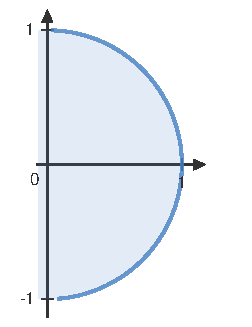
\includegraphics[width=\linewidth]{fig3.pdf}
    \end{minipage}
\end{Example}
